% Please use the skeleton file you have received in the
% invitation-to-submit email, where your data are already
% filled in. Otherwise please make sure you insert your
% data according to the instructions in PoSauthmanual.pdf
\documentclass{PoS}

\title{Summary of Working Group 4 : mixing and mixing-related $CP$ violation in the $B$ system}

\ShortTitle{All SM everything}

\author{\speaker{Alessandro Gaz}\\
        Nagoya\\
        E-mail: \email{gaz@hepl.phys.nagoya-u.ac.jp}\\
        \speaker{Vladimir V. Gligorov}\thanks{I would like to thank my mum, dad, and trade union representative for their support. Couldn't have done it without you!}\\
        LPNHE, Universit\'{e} Pierre et Marie Curie, Universit\'{e} Paris Diderot, CNRS/IN2P3, Paris, France\\
        E-mail: \email{vgligoro@lpnhe.in2p3.fr}\\
        \speaker{Dean Robinson}\\
        Cincinatti\\
        E-mail: \email{dean.robinson@uc.edu}\\
        }

%\author{Another Author\\
%        Affiliation\\
%        E-mail: \email{...}}

\abstract{$B$ mesons mix and in mixing do wonderful and amazing things.}

\FullConference{9th International Workshop on the CKM Unitarity Triangle\\
		28  November - 3 December 2016\\
		Tata Institute for Fundamental Research (TIFR), Mumbai, India}


\begin{document}

\section{Introduction}
Neutral beauty mesons can oscillate into their antiparticles through the exchange of $W^\pm W^\mp$ pairs, so that the 
physical states (those with well defined masses and lifetimes) are admixtures of the flavour eigenstates. This gives
rise to both mass ($\delta m_{(d,s)}$) and width ($\Delta\Gamma_{(d,s)}$) splittings in the $B^0_d$ and $B^0_s$ systems, as well
as two types of related $CP$ violation. The first, $CP$ violation in mixing, occurs when the meson and antimeson have different
probablities to oscillate into each other, and is predicted to be very close to zero in the Standard Model (SM) with a very
small theoretical uncertainty. The second, $CP$ violation in the intereference of decay and mixing, occurs when both the meson
and antimeson can decay to the final state, and the decay paths with and without intermediate mixing interfere. This kind of $CP$
violation is highly sensitive to the imaginary component of the CKM matrix and its absolute size depends on the final state in question.

Aside from their intrinsically fundamental nature, measurements of mass and width splittings and mixing-related $CP$ violation are
of great interest because many of the observables can be predicted very precisely in the SM, and because new particles or force-carriers
beyond the SM (BSM) can alter these predictions in experimentally observable ways. Many different experimental collaborations have contributed
to our understanding of mixing in the $B$ system, from the inital discovery of $B$ mixing by the ARGUS collaboration~\cite{}, to precise measurements
of $\delta m_{(d,s)}$ and the CKM-angles $\alpha$ and $\beta$ at the b-factories and Tevatron~\cite{}, to recent precise measurements
of $\phi_s$, $\Delta\Gamma_s$, and first precise mixing-related measurements of the CKM-angle $\gamma$ at ATLAS, CMS, and LHCb~\cite{}. At the same
time, great progress has been made in making more precise theoretical predictions of the SM values of many of these quantities, making
these experimental measurements sensitive probes of BSM physics.

The remainder of this document covers the current status of experimental measurements and theory predictions for each observable of
interest, as well as their near-term outlook. Section~\ref{sec:phisdgs} covers measurements of $\phi_s$ and $\Delta\Gamma_s$, section~\ref{sec:dmdgd} 
mesurements of $\delta m_{(s,d)}$. Section~\ref{sec:photpol} covers the measurements of photon polarization in radiative decays, while
sections~\ref{sec:alpha}~to~\ref{sec:gamma} cover measurements of the CKM angles $\alpha$, $\beta$, and $\gamma$, respectively.
For historical reasons, measurements of $CP$ violation in neutral meson mixing are covered in the proceedings of WG~\cite{}. Finally we conclude,
and discuss the medium to long-term outlook for mixing-related measurements in the $B$ system.



\section{Measurements of $\phi_s$}


\section{Measurements of $\Delta\Gamma_{(d,s)}$}

\section{Measurements of $\Delta m_{(d,s)}$}


\section{Measurements of the CKM angle $\alpha$}
\label{sec:alpha}

\section{Measurements of the CKM angle $\beta$}
\label{sec:beta}

While the world average~\cite{HFAG} of $\beta$ is still dominated
by the BaBar~\cite{} and Belle~\cite{} measurements, LHCb also contributes~\cite{LHCb-PAPER-2012-035} and can be expected
to reach the BaBar and Belle individual sensitivities once Run~II data and
improvements in flavour tagging are included in the analysis. LHCb has also measured~\cite{LHCb-PAPER-2015-005}
$CP$ violation in $B^0_s \to J/\psi K^0_S$ decays,
which can help to constrain the size of penguin contributions to the measurement
of $\beta$ from $B^0 \to J/\psi K^0_S$, as well as the $CP$ violating parameters in
$B^0 \to D^+ D^-$ decays, which can also be interepreted in terms of constraints on $\beta$.
The current world average of measurements of $B^0 \to D^+ D^-$ is shown in Fig.~\ref{b2ddwa}; 
interestingly while all measurements are compatible with each other, the LHCb measurement
does not confirm the maximal (within uncertainty) Belle measurement of $S$.

\begin{figure}
  \begin{center}
    \begin{tabular}{c c}
      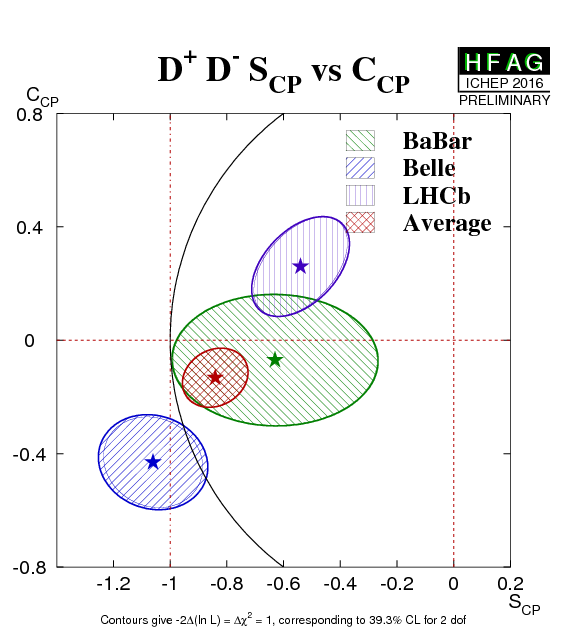
\includegraphics[height=7.5cm]{figs/D+D-S_CPvsC_CP.png} &
    \end{tabular}
  \end{center}
  \vspace{-0.5cm}
  \caption{\label{b2ddwa}World average of time-dependent $CP$ observables in $B^0 \to D^+ D^-$, reproduced from HFAG~\cite{HFAG}.}
\end{figure}

The BaBar and Belle Collaboration obtained the first observation of $CP$-violation
in the channels $B^0 \to D^{(*)}_{CP} h^0$, where $h^0$ is a light unflavored neutral
meson, by combining their final datasets \cite{babar_belle_D0h0}. Neglecting the
very small contribution from the $CKM$ suppressed amplitude $b \to u\bar{c}d$,
the time dependent analysis is sensitive to $\sin(2\beta)$. A joint likelihood,
sharing the same physics parameters but independent background modeling parameters,
the two experiments find:
\begin{eqnarray}
-\eta_f S & = & +0.66 \pm 0.10 (\mbox{stat}) \pm 0.16 (\mbox{syst}), \\
C & = & +0.02 \pm 0.07 (\mbox{stat}) \pm 0.03 (\mbox{syst}), 
\end{eqnarray}
with the significance of the observation beeing 5.4 standard deviations. 

\section{Measurements of the CKM angle $\gamma$}
\label{sec:gamma}
Measurements of the CKM angle $\gamma$ require the interference of $b\to u$ and $b\to c$ transitions.
Such interference can occur in the decays of charged as well as neutral $B$ hadrons, in tree-dominated
transitions as well as transitions where both tree and loop diagrams contribute.
The measurement of $\gamma$ from the tree-dominated decays of $B^\pm$ mesons, covered in the 
proceedings of WG5~\cite{WG5PROC}, has a particular importance as it allows a purely tree-level\footnote{Higher order box corrections~\cite{ZupanBrodGamma}
only enter at $\delta\gamma/\gamma \approx 10^{-7}$, well beyond any current or future experimental sensitivity.}
determination of the apex of the unitarity triangle, and therefore a test of the self-consistency of the CKM
mechanism of $CP$ violation when compared with determinations of $\alpha$ and $\beta$ in transitions where
both tree and loop diagrams contribute. It is also, however, possible to measure $\gamma$ by exploiting
$CP$ violation in the interference of mixing and decay of neutral $B$ mesons. These time-dependent determinations
of $\gamma$ are particularly powerful in the case of $B^0_s$ mesons, because the large width difference between
the light and heavy $B^0_s$ eigenstates makes additional $CP$ observables available compared
to the $B^0$ system and allows for a determination of $\gamma$ with fewer ambiguities. 
%While these are not
%strictly tree-level determinations, as the mixing of neutral $B$ mesons

A particularly powerful time-dependent measurement of $\gamma$, described in detail in these proceedings~\cite{DSKPROC}, utilizes the decay $B^0_s \to D^\pm_s K^\mp$.
In this case the $b\to u$ and $b\to c$ transitions are both of order $\lambda^3$, leading to large interference, and
the large value of $\Delta\Gamma_s$ allows for a determination of $\gamma$ with only a twofold ambiguity. 
The preliminary result obtained with the full Run~I LHCb dataset, which shows $3.6\sigma$ evidence for $CP$-violation in this mode, is
\begin{equation}
\gamma      = (127_{-22}^{+17})^\circ\,,\phantom{space}
\strong = (  358_{-16}^{+15})^\circ\,,\phantom{space}
\rdsk   = 0.37_{-0.09}^{+0.10}\,,\phantom{space}
(68.3\% \textrm{CL})\phantom{space}  
\end{equation}
\begin{equation}
\gamma      = (127_{-50}^{+33})^\circ\,,\phantom{space}
\strong = (  358_{-33}^{+31})^\circ\,,\phantom{space}
\rdsk   = 0.37_{-0.19}^{+0.19}\,,\phantom{space}
(95.4\% \textrm{CL})\phantom{space}  
\end{equation}
where $\strong$ is the $CP$-conserving angle between the $b\to u$ and $b\to c$ transitions,
$\rdsk$ is the amplitude ratio of the interfering diagrams, and the intervals for the angles are expressed modulo $180^\circ$.
The uncertainties are a combination of statistical and systematic ones; the statistical uncertainties dominate
and all systematic uncertainties are expected to scale with luminosity for the foreseeable future.

While not the most sensitive single-mode determination of $\gamma$, $B^0_s \to D^\pm_s K^\mp$ plays a similar
role in the overall LHCb combination~\cite{LHCb-PAPER-2016-032} of $\gamma$ to that of the GGSZ measurement. Because of their twofold ambiguity, these measurements
select the ``correct'' solution among the ones allowed by the most precise ADS/GLW measurement~\cite{LHCb-PAPER-2016-003}. For this reason the determination
of $\gamma$ from $B^0_s \to D^\pm_s K^\mp$, which is only possible at LHCb, will remain a key measurement for both the current
and upgraded LHCb detectors. LHCb is also pursuing a measurement of time-dependent $CP$-violation in
the decay mode $B^0 \to D^\pm \pi^\mp$, described in these proceedings~\cite{BDPIPROC}, but no results are available yet.
This measurement, previously performed by BaBar~\cite{Aubert:2005yf}, \cite{Aubert:2006tw} and Belle~\cite{Bahinipati:2011yq}, \cite{Ronga:2006hv}
is much less sensitive than $B^0_s \to D^\pm_s K^\mp$, both because of smaller interference and because
the small value of $\Delta\Gamma_d$ leads to fewer accessible $CP$-observables. The much smaller $CP$ asymmetry
also makes this measurement particularly sensitive the asymmetries in the flavor tagging of $B^0$ and $\bar{B^0}$ mesons.
Nevertheless, it is expected that both LHCb and Belle-II will carry out this measurement in the future.

\section{Conclusion}
The last two decades have seen an enormous progress in the understanding of $B$ meson mixing and mixing-related
$CP$ violation, both in terms of precise experimental measurements of the underlying constants of nature and in terms of 
the theoretical understanding of their values within the Standard Model. We now have precise measurements 
or stringent limits on the mass splitting, width splitting, and mixing phase in both the $B^0$ and $B^0_s$ systems,
while mixing-induced $CP$ violation is being precisely measured or constrained in an ever increasing number of final states.
With the LHCb upgrade~\cite{} and Belle~II~\cite{Abe:2010gxa} detectors due to come online in the next years, and none of the fundamental measurements
yet systematically limited, we can expect this progress to continue. Important contributions, particularly as regards
$\phi_s$ and $\Delta\Gamma_d$ can also be expected from CMS and ATLAS, and in particular it is realistic to expect the $B^0_s$ mixing
phase to be measured significantly away from zero even at the Standard Model value within the next decade. Recently
the LHCb collaboration has proposed a Phase~II upgrade of its detector~\cite{}, to take data in the HL-LHC period,
which would collect 300~fb$^{-1}$, and enable not only a single-experiment observation of $\phi_s$ in multiple independent
decay modes, but also make it possible to see evidence for a non-zero $\Delta\Gamma_d$ at its Standard Model value.
\textbf{ADD SOME WORDS ON THEORY TO FINISH THIS OFF}
%Particle physics is now roughly where the French monarchy was in 1788, and CERN is Versailles. But who will be our Robespierre?


%\bibliographystyle{PoS}
\bibliography{skeleton}

\end{document}
